It has been more than 30 years, since it was proven, that already simple neural network architectures can in fact be \emph{universal approximators} \cite*{ffnUnversalApproximator}. 
That means that if a problem can be formulated as a mathematical function, this function can be approximated by a neural network.
This has huge consequences, because if input and output are encoded digitally in a predefined format, \emph{all} mappings between these can be formulated in form of a mathematical function. 
Be it only the trivial one, that maps each input encoding to the desired output encoding.
Because of that, seemingly impossibly complex problems can be tackled now days. 

Part of the experimentation in the thesis will focus on the application of a select breed of neural networks on the \emph{image classification task}.
This is not a novel problem, but one that has been tried and solved by many teams of researchers. 
The gist is, to build a neural network that can label the things pictured on some kind of image.
In our case, an even simpler version of the problem will be considered. 
The only job of the network is, to select one of $N$ predefined labels, that describe the picture best.

The architecture of the network can be viewed generalized in \autoref{fig:image-classification-general}.

\begin{figure}[htbp]
    \centering
    \makebox[\textwidth][c]{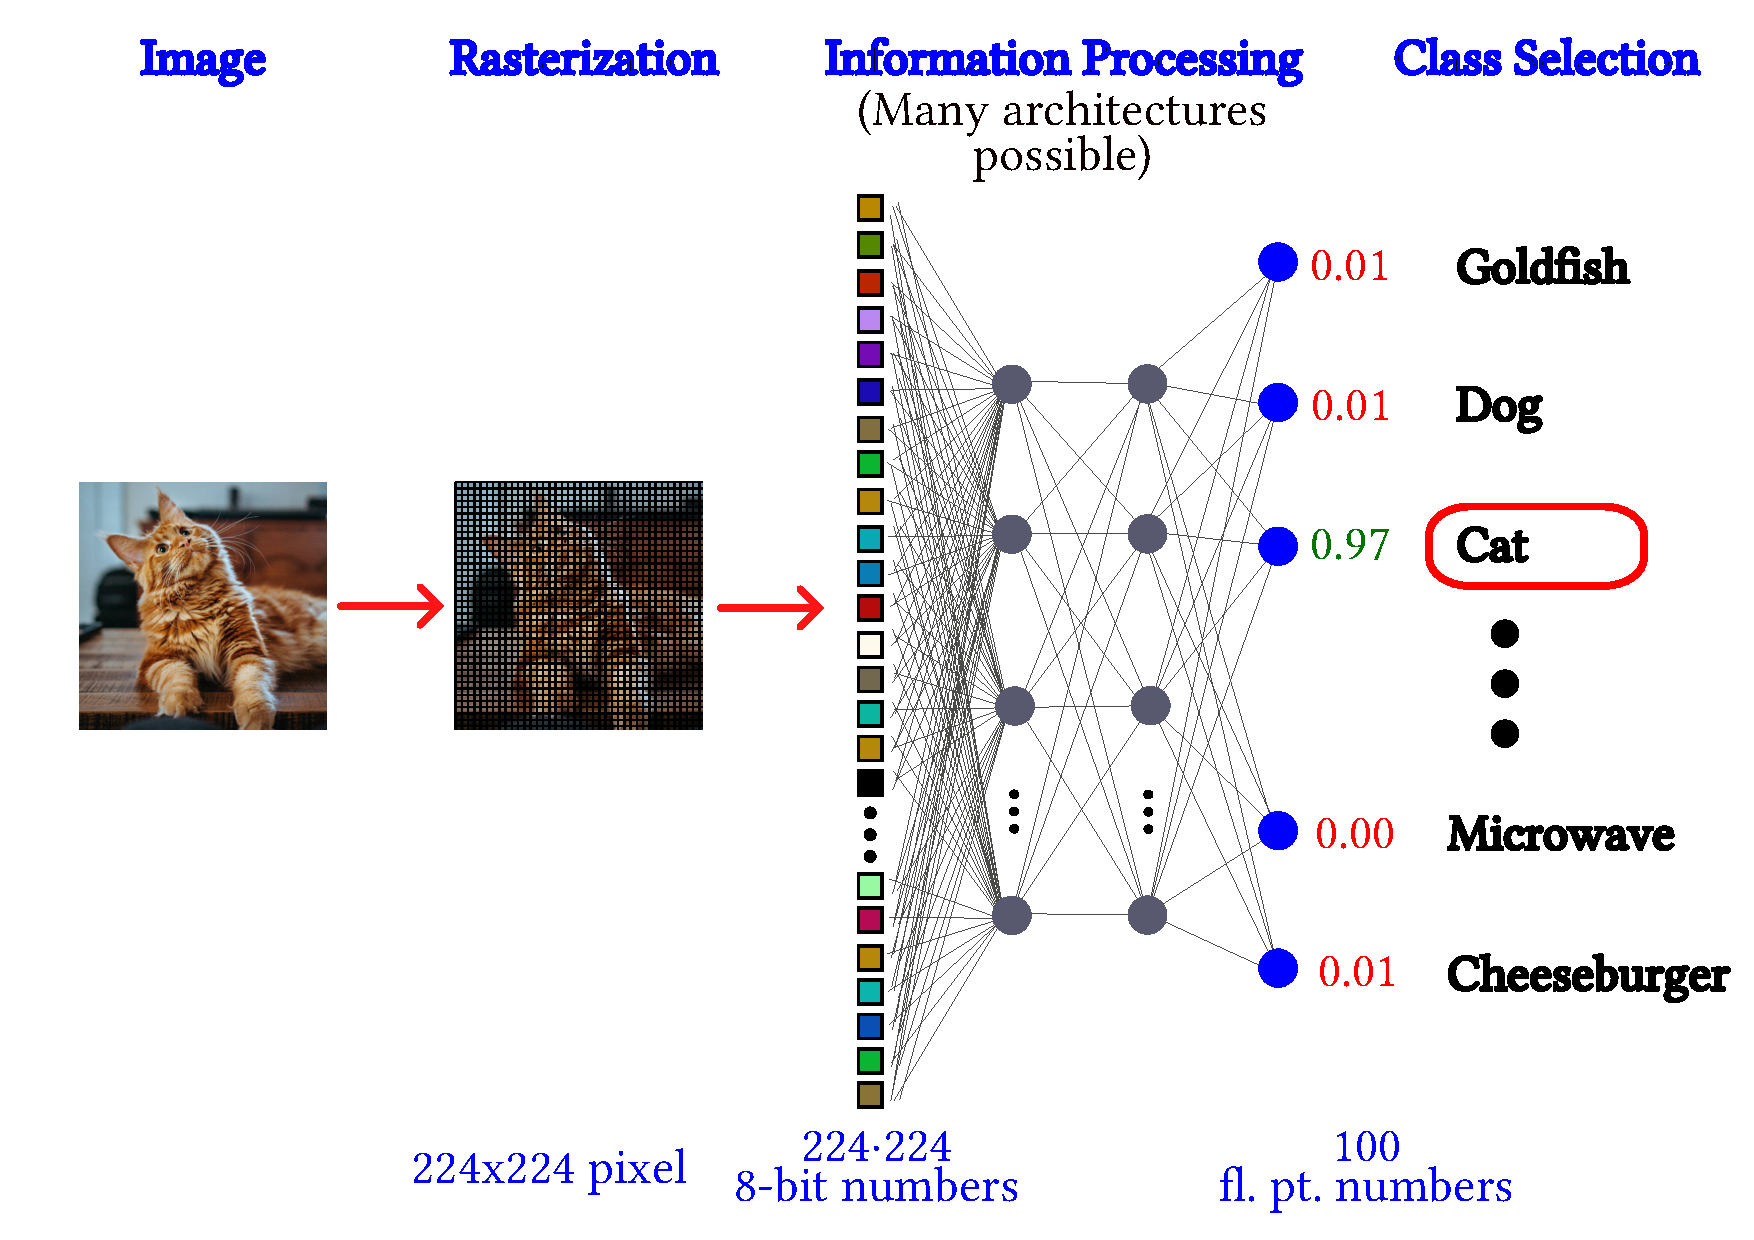
\includegraphics[width=\textwidth]{./theory/cs/image-classification/process.pdf}}
    \caption{Generalized schema of the image classification pipeline used in the experiments portion of this thesis.
        The image gets rasterized, resized to 224$\times$224 pixel and 8 bit color depth per each of the three color channels. Then the image is normalized, reshaped into vector form and processed from there. The MLP in this image is only a placeholder. Many of the later discussed neural network architectures treat the reshaping, casting and processing differently. The output for all networks needs to be in form of 100 floating point numbers. the one closest to one gets selected as the networks choice. The class name, the index represents can then be looked up.
        Cat image from \cite{catPhoto}.
    }
    \label{fig:image-classification-general}
\end{figure}

The aforementioned trivial mapping of inputs to outputs is obviously not feasable in reality, as there would need to be $256^{224\cdot 224} \approx \SI[]{7e120835}[]{}$ possible cases. Most of which do not even make sense in terms of the predefined categories or even define a realistically possible image.

In order to solve the problem, the mapping function is \emph{approximated} with a neural network. 

To train the network, a pre-labeled set of training images is passed through the network, the results are compared to the labels and the error is used to iteratively update the network with use of the \emph{backpropagation algorithm} \cite{machineLearningMitchell}, therefore improving the performance of the network in the next step.

A big challenge in training these kinds of networks is getting a sufficient amount of labeled training data. 
Today a lot of publicly available, high quality datasets exist for download. 
In this case, the \emph{CIFAR-10} \cite{cifarDataset} dataset was used for the first steps in the methods. 
A subset of \emph{100 classes} from the \emph{ImageNet} \cite{imagenetDataset} dataset was used in the experiments that were used to evaluate the general functionality of the explored network architectures.
The subset of chosen classes can be viewed at \cite{selfComputerScience} \filepath{/managing\_imagenet\_data/used\_synsets.txt}.

In the task, the \emph{accuracy} describes the percentage of validation images whose label was guessed correctly by the network. It is not allowed to use the validation images during training. That way, the network only would need to memorize a tiny amount of images to perform good on the test. This is undesirable behavior, as the general idea is to teach the network to be able to classify previously unseen images in the right way. The \emph{training accuracy} is the analogous value, but calculated for the training images (that \emph{are} used during training. Because of that, this accuracy is often way higher).
The \emph{top-3-accuracy} is the percentage of validation images, for that the correct label was among the top three highest valued choices of the network. The same is true analogously for the \emph{top-5-accuracy}.